\title{Definition of the interannual experiment <CONFIG>-<CASE>, <FYEAR>-<LYEAR>}
\author{
        Albanne Lecointre, Jean-Marc Molines, Bernard Barnier \\
        MEOM - LEGI - CNRS \\
        LEGI-DRA-21-10-2011
}
%\date{\today}
\date{ }

\documentclass[12pt]{article}

\usepackage{graphicx}
\usepackage{url}
\usepackage{float}
\usepackage[french,english]{babel}
\usepackage{verbatim}
\usepackage[T1]{fontenc}
\usepackage[top=2cm, bottom=2cm, left=2cm, right=2cm]{geometry}
\usepackage{textcomp}
\usepackage{color}
\usepackage{hyperref}



\newcommand{\figwidth}{\linewidth}

\begin{document}

\maketitle

\section*{Introduction}

This report describes in details the ORCA12.L46-MAL95 simulation performed in the frame of the DRAKKAR project. This run is the first ORCA12 simulation computed at MEOM (LEGI, CNRS). The mesh is an ORCA grid 1/12\degres \enspace at equator, with partial-steps, 46 levels Drakkar type. It is a following of the Kiel (IFM Geomar) ORCA12.L46-K001 run (started in 1978 from Levitus) but we change the forcing fields from CORE2 to ERA-interim. The purposes of this run are thus to learn how to run such a big model and to perform a sensitivity experiment between CORE2 (K001) and ERA-interim forcing. The code is based on version NEMO 3.2.2.

This report is organized in different sections. The first one deals with the details of the numerical code, the parametrizations used and the forcing issues. The second section describes the model configuration, e.g. the model grid and the input data of the model. A third section is dedicated to the technical details of the production of the run and give some informations about the computing performance. Finally, the last section gives some elements of validation of the run.

%---------------------------------------------------------------------------------------------------

\section{Numerical code}

%---------------------------------------------------------------------------------------------------

\subsection{Overview}

This experiment was performed with version 3.2.2 of NEMO. CPP keys used for compilation are:

\begin{center}
\begin{tabular}{|l|l|}
\hline
\textbf{CPP key name} & \textbf{Action:} \\
\hline
key\_orca\_r12        & ORCA12 horizontal grid with 46 vertical levels \\
\hline
key\_dynspg\_flt      & Filtered free surface \\
\hline
key\_zdftke           & Tke turbulent closure for vertical diffusion \\
\hline
key\_dtatem           & Initialize model from temperature climatology \\
\hline
key\_dtasal           & Initialize model from salinity climatology \\
\hline
key\_traldf\_c2d      & 2D horizontal dependency on lateral diffusivity \\
\hline
key\_dynldf\_c2d      & 2D horizontal dependency on lateral viscosity \\
\hline
key\_ldfslp           & Compute isopycnal slopes \\
\hline
key\_dimgout          & Use temporary binary files for mpp output \\
\hline
key\_mpp\_mpi         & Parallel processing using MPI library \\
\hline
key\_lim2             & Use LIM2 ice model \\
\hline
key\_trabbl\_dif      & Use BBL enhanced diffusion on tracers \\
\hline
\end{tabular}
\end{center}

%---------------------------------------------------------------------------------------------------

\subsection{Ocean details}

\subsubsection{Vertical physics}

\paragraph{TKE scheme \\}

TKE is used to determine the vertical diffusion coefficient. The relevant namelist data are indicated below. Note that in this version, a non-standard treatment is performed on ice-covered area: (a) The background avt coefficient is divided by 10 under ice. (b) There is no background of Tke under ice. (c) The coefficient for surface input of tke (ebb) is reduced from 60 (open ocean) to 3.75 (ice covered regions). (d) Lang-Muir cells parametrization is turned off below ice.

\scriptsize
\verbatiminput{./namelist-blocks/namzdf.txt}
\verbatiminput{./namelist-blocks/namzdf_tke.txt}

\normalsize

%--------------------------------------------------------------------------------------

\subsubsection{Horizontal physics}

\paragraph{Tracers \\}

We use a laplacian isopycnal diffusivity for tracers. The diffusivity is proportionnal to the local grid size (it decreases poleward). The horizontal eddy diffusivity for tracers is reduced to 125 $m^2/s$ for ORCA12 configuration (compared to ORCA025 : 300 $m^2/s$).

\scriptsize
\verbatiminput{./namelist-blocks/namtra_ldf.txt}

\normalsize

\paragraph{Momentum \\}

We use a bi-harmonic viscosity for the lateral dissipation. Note that in the ORCA12 configuration, the viscosity is reduced by a factor 14 compared to ORCA025 configuration. The viscosity is proportionnal to the grid size power 3.

\scriptsize
\verbatiminput{./namelist-blocks/namdyn_ldf.txt}

\normalsize

%--------------------------------------------------------------------------------------

\subsubsection{Bottom Boundary Layer}

We used bottom boundary layer parametrization (\cite{Beckmann1997}). Only diffusive (not advective) BBL parametrization is used for tracers, and no BBL advection parametrization for momentum \footnote{We don't apply the improvement on BBL parametrization proposed in \cite{Hervieux} as for MJM95 simulation.}.

\scriptsize
\verbatiminput{./namelist-blocks/nambbl.txt}

\normalsize

\subsubsection{Surface boundary conditions}

The surface boundary conditions are prescribed to the model using the CORE bulk formulation. The initial part of the run: K001 (\cite{Scheinert}), performed by IFM-Geomar (Kiel) group from 01/01/1978 to 31/12/1988 (and after...) used CORE II forcing.
The following part of the run: MAL95, from 01/01/1989 to end (31/12/2007), was forced by ERA-interim reanalysis products (just as ORCA025.L75-MJM95). The data set includes 4 turbulent variables (u10, v10, t2, q2) given every 3 hours, 2 radiative fluxes variables (radsw, radlw), 2 fresh water flux variables (total precipitations, snow) and the total cloud cover (tcc), all these last variables given as daily averaged.

\scriptsize
\verbatiminput{./namelist-blocks/namsbc.txt}

\verbatiminput{./namelist-blocks/namsbc_core.txt}

\normalsize

\paragraph{Radiative flux and precipitation corrections \\}

The radiative fluxes (both long wave and short wave) and precipitation exhibit unacceptable bias. Therefore a specific correction has been implemented by \textcolor{blue}{Garric (reference paper ?)} in order to improve those fluxes and precipitation. For radiative fluxes, a correction factor based on the comparison between ERA-interim fluxes and satellite fluxes products (GEWEX) is computed. For precipitation, the correction uses large scale GPCP product. These corrections required some change in the code as described here. Basically, the idea is to apply a 2D scaling coefficient to the large scale features of the radiative fluxes and precipitation. Original fields are band-pass filtered to separate large scales and small scales, using a shapiro filter, applied 250 times during the period 1989-1991 and enhanced to 600 times during the period 1992-2007 (which reduced the performance rate of the model computing by 5\%). The correction is applied to the large scale and then the small scale is added to produce the radiative fluxes and precipitation for the model. Finally we applied a scale factor to this radiative flux correction in Arctic and Southern Ocean (solar heat flux: 70\% in the Arctic and 80\% in the Southern Ocean; long wave heat flux: 110\% in the Arctic and Southern Ocean). For precipitation, we only applied the correction between 30\degres S and 30\degres N, with a buffer zone between 30\degres N/S and 40\degres N/S. No correction is applied northward of 40\degres N and southward of 40\degres S.


\paragraph{Light penetration algorithm according to ocean color \\}

In this simulation we use a non-standard parametrization of the penetration of the solar flux in the ocean, modulated by the chlorophyll concentration, deduced from satellite (SeaWIFS ocean color products) ocean color monthly climatology developed by \cite{Lengaigne2007}. In this solar radiation penetration formulation, visible light is split into three wavebands: blue (400-500nm), green (500-600nm), red (600-700nm).

\scriptsize
\verbatiminput{./namelist-blocks/namtra_qsr.txt}

\normalsize

\paragraph{Diurnal Cycle on solar fluxes \\}

In this run and contrary to ORCA025.L75-MJM95, there is no parametrization of the diurnal cycle on the solar flux. We don't implement it in order to respect the choice made in the K001 previous run.

\paragraph{River Run-off \\}

For K001 and MAL95 simulations, the coastal and river run-off data is inferred from the file \footnote{provided by MERCATOR and Anne-Marie Trguier} runoff\_coast1pt\_ant3pt\_isl20\_obtaz\_1m\_ORCA12\_correctAMZ\_200610\_lbclnk.nc. Contrary to ORCA025.L75-MJM95, there is no specific treatment at rivers mouths.

\scriptsize
\verbatiminput{./namelist-blocks/namsbc_rnf.txt}

\normalsize

\paragraph{SSS restoring strategy \\}

We used standard Sea Surface Salinity restoring toward Levitus, with a time scale of 60 days/10 meters (considered as rather strong). There is no SSS damping under sea-ice. 
A limitation is applied to the restoring term ($|Sobs - Smodel| \leq 0.5 PSU$), to limit the damping in regions with large variations of the SSS, like in boundary currents or the NAC. 
Then we apply ERP bounding on this resulting SSS (limitation at 4 mm/day as it was the case in ORCA025.L75-MJM95)\footnote{Note that the Kiel run only use the limitation on absolute SSS, 
not the ERP bounding (\textit{ln\_sssr\_bnd=.false.}). 
We applied this ERP bounding by error... 
And it seems to have an impact because some of the output fields have a \textit{sowafldp} (surface water flux related to SSS damping) range between $-4.62963.10^{-5}$ and $4.62963.10^{-5} kg/m^2/S$}, 
which exactly corresponds to 4mm/day assuming 1 water $m^3=10^3 Kg$.
There is no enhancement of the restoring term in the Mediterranean Sea like in ORCA025.L75-MJM95. 
In the next ORCA12 runs we have to decide which regional parametrization for salinity restoring to implement.

\scriptsize
\verbatiminput{./namelist-blocks/namsbc_ssr.txt}

\normalsize

\subsubsection{Lateral boundary condition}

The lateral momentum boundary condition was set to 0.5 (partial slip condition), with respect to K001. Note that it exists a sensitivity test concerning this shlat boundary condition: ORCA12.L46-MAL950 run was performed during 3 years (1989-1991) but with a free slip condition (shlat=0). This (too ?) short 3-year experiment does not show any clear improvement in the Gulf Stream detachment.

\scriptsize
\verbatiminput{./namelist-blocks/namlbc.txt}

\normalsize

\subsubsection{Tracer damping strategy}

There is no 3D tracer damping at all (nowhere in the ocean). Particularly there is no 3D restoring in the Gulf of Cadiz, leading to poor Mediterranean Waters in the Atlantic.

%---------------------------------------------------------------------------------------------------

\subsection{Ice details}

\subsubsection{EVP rheology}

The model used the LIM2 model (without the Elasto-Visco-Plastic rheology). The ice-ocean coupling is done every 6 model steps.

\subsubsection{Thermodynamics}

The standard LIM2 thermodynamics is used. The only change with respect to the standard code is the use of cloud cover files (synoptic) instead 
of a standard constant value for nebulosity. It has an impact on the net shortwave radiation which is not absorbed in the thin surface 
layer and penetrates inside the ice cover.

Note that the ice thickness for lateral accretion (\textit{hiccrit}) is 0.6 in the Northern and Southern Hemisphere.

\scriptsize
\verbatiminput{./namelist-blocks/namicedyn.txt}

\verbatiminput{./namelist-blocks/namicethd.txt}

\normalsize

%---------------------------------------------------------------------------------------------------

\section{Model configuration}

\subsection{Bathymetry}

The bathymetry used for this run is a merge of etopo2 for the deep ocean and gebco1 for shallow areas (old bathymetry file - bathymeter\_p083\_05.nc - by error). 
The minimum depth in the model was set to 14.3 meters (3 vertical levels with partial step condition).

\subsection{Horizontal grid}

The horizontal grid is the standard ORCA12 tri-polar grid (4322 x 3059 grid points). The 1/12\degres \enspace resolution corresponds to the equator (10km). Resolution increases poleward: 5km at 60\degres, 3.5km at 75\degres \enspace (the grid size is scaled by the cosine of the latitude, except in the Arctic, of course).

\subsection{Vertical grid}

The vertical grid has 46 levels, with a resolution of 6m near the surface and 250m in the deep ocean.

\subsection{Initial conditions}

\subsubsection{Ocean}

The original K001 simulation (\cite{Scheinert}) \textcolor{blue}{(does it exist a more complete or more recent reference ?)} started from rest in 1978, with initial climatological temperatures and salinities. The used climatology was a merge of the Levitus 1998 climatology, patched with PHC2 for the Arctic regions and Medatlas for the Mediterranean Sea. The ORCA12.L46-MAL95 simulation is initialized from restart files provided by the Kiel group in 1989, January $1^{st}$. This restart file was 46.8 GB (ocean) and 5.0 GB (ice) : we had to stripe it on 20 disks (with JADE lfs commands) to reduce the reading time.

\subsubsection{Ice}

The Kiel run (K001) used the ice standard initialisation from Levitus SST climatology, with following parameters:
\begin{itemize}
 \item 3m (1m) sea-ice width in the north (south);
 \item 0.5m (0.1m) snow width in the north (south);
 \item 5\% (10\%) leads area in the north (south).
\end{itemize}

\scriptsize
\verbatiminput{./namelist-blocks/namiceini.txt}

\normalsize

The ORCA12.L46-MAL95 simulation started from an ice restart file from this K001 simulation in 1989, January $1^{st}$.

\subsection{Miscellaneous}

During the entire run performed at MEOM-LEGI (1989-2007) we used a time step of 360 sec. But the time step used at the beginning of the K001 run performed at IFM-Geomar (Kiel) was 72 sec for the first 5 days, and then increased progressively to 144 sec for days 6-15, 300 sec for days 16-20 and 360 sec after. Robert-Asselin filter parameter was increased to 0.2 for the first 10 days (K001) to avoid overshoots, and then reduced to the configuration default value 0.1. We kept this default value for the entire ORCA12.L46-MAL95 run over the period 1989-2007.

%---------------------------------------------------------------------------------------------------

\section{Run production}

\subsection{Integration and computing performance}

The run started January, $1^{st}$, 1989 (restart \footnote{To restart we had to stripe the 46.8GB (ocean) + 5.0GB (ice) restart files from K001 on 20 disks.} from K001, which started January, $1^{st}$, 1978) and ended December, 31$^{st}$, 2007, corresponding to the available ERA-interim forcing field. Note however that we don't compute 2008-2009 (whereas ERA-interim forcing field is available at this period), because the Kiel run (K001) ended in 2007. The run was performed at CINES HPC center in Montpellier, using 2032 cores of the SGI Altix ICE 8200 cluster (Jade). The domain decomposition used is 46 x 60 cores along x- and y- directions respectively for a total of 2032 computing core (land domain were eliminated). Each core computes 96 x 53 grid points. The placement strategy implemented (no ``depopulated core condition'' but ``away-neighbour placement'') allowed us to reach computing performance of 56 000 CPU hours per simulated year (28 elapsed hours per simulated year). The total CPU cost of this 19-year simulation is 1 091 162 CPU hours. More details about performance computing strategy can be found in \cite{Lecointre2011} and on demand at \href{mailto:albanne.lecointre@legi.grenoble-inp.fr}{albanne.lecointre@legi.grenoble-inp.fr}. We performed 6-month runs with a 15h00 walltime, with a restart file frequency of 6 months \footnote{Finally, only 1-year restart files were archived.}.

\subsection{Model output}

Model output is done as 5-days averages. Then monthly and annual means are computed in the post processing. The output size represents 1.9Tb per year (for 5-day + monthly and annual means). We also computed two climatologies over the periods 1998-2007 (the last 10 years) and 2003-2007 (for comparison with T321 Mercator run).

\subsection{Journal of the run}

A detailed journal of the run production is available on demand at \href{mailto:albanne.lecointre@legi.grenoble-inp.fr}{albanne.lecointre@legi.grenoble-inp.fr}.

%---------------------------------------------------------------------------------------------------

\section{Validation}

The <CONFIG>-<CASE> validation that is presented here is extracted from the monitoring of the experiment, available on demand on the Drakkar web site (contact \href{mailto:bernard.barnier@legi.grenoble-inp.fr}{bernard.barnier@legi.grenoble-inp.fr}).

\subsection{Mean state of the ocean (<MFYEAR>-<MLYEAR>)}

We present here maps of the time mean of the major ocean variables (temperature, salinity, sea surface height, barotropic transport streamfunction and meridional overturning circulation).

\begin{figure}[H]
\begin{center}
%\includegraphics[width=15cm]{./figs_monitor/<CONFIG>_Tgl_0_<MFYEAR>-<MLYEAR>-<CASE>.eps}
\caption{Mean Sea Surface Temperature over the period <MFYEAR>-<MLYEAR>. Colours indicate the SST in \degres C, and contour lines indicate the sea ice thickness.}
\end{center}
\end{figure}

\begin{figure}[H]
\begin{center}
%\includegraphics[width=15cm]{./figs_monitor/<CONFIG>_Sgl_0_<MFYEAR>-<MLYEAR>-<CASE>.eps}
\caption{Mean Sea Surface Salinity over the period <MFYEAR>-<MLYEAR>. Colours indicate the SSS, and contour lines indicate the sea ice thickness.}
\end{center}
\end{figure}

\begin{figure}[H]
\begin{center}
%\includegraphics[width=15cm]{./figs_monitor/<CONFIG>_SSHGLp_0_<MFYEAR>-<MLYEAR>-<CASE>.eps}
\caption{Mean Sea Surface Height over the period <MFYEAR>-<MLYEAR>. Colours indicate the SSH in meters, and contour lines indicate the sea ice thickness.}
\end{center}
\end{figure}

\begin{figure}[H]
\begin{center}
%\includegraphics[width=15cm]{./figs_monitor/<CONFIG>_PSI_ATLN_<MFYEAR>-<MLYEAR>-<CASE>.eps}
\caption{Mean Barotropic Streamfunction over the period <MFYEAR>-<MLYEAR>. Contours by 10 Sv, negative values are shaded.}
\end{center}
\end{figure}

\begin{figure}[H]
\begin{center}
%\includegraphics[width=10cm]{./figs_monitor/<CONFIG>_OVT_glo_<MFYEAR>-<MLYEAR>-<CASE>.eps}
%\includegraphics[width=10cm]{./figs_monitor/<CONFIG>_OVT_atl_<MFYEAR>-<MLYEAR>-<CASE>.eps}
\caption{Mean Overturning over the period <MFYEAR>-<MLYEAR>. Top: Global Ocean, bottom: Atlantic Ocean. Contours by 2 Sv.}
\end{center}
\end{figure}

\subsection{Temperature and salinity CLASS1-1}

The 10-year mean temperature difference with Levitus 2009 climatology at various depths (0m, 100m, 500m) is shown below.

\begin{figure}[H]
\begin{center}
\begin{minipage}{0.47\linewidth}
%\includegraphics[width=7cm]{./figs_monitor/<CONFIG>_difTgl_k1_<MFYEAR>-<MLYEAR>-<CASE>.eps}
\end{minipage}
\hfill
\begin{minipage}{0.47\linewidth}
%\includegraphics[width=7cm]{./figs_monitor/<CONFIG>_difSgl_k1_<MFYEAR>-<MLYEAR>-<CASE>.eps}
\end{minipage}
\begin{minipage}{0.47\linewidth}
%\includegraphics[width=7cm]{./figs_monitor/<CONFIG>_difTgl_k12_<MFYEAR>-<MLYEAR>-<CASE>.eps}
\end{minipage}
\hfill
\begin{minipage}{0.47\linewidth}
%\includegraphics[width=7cm]{./figs_monitor/<CONFIG>_difSgl_k12_<MFYEAR>-<MLYEAR>-<CASE>.eps}
\end{minipage}
\begin{minipage}{0.47\linewidth}
%\includegraphics[width=7cm]{./figs_monitor/<CONFIG>_difTgl_k19_<MFYEAR>-<MLYEAR>-<CASE>.eps}
\end{minipage}
\hfill
\begin{minipage}{0.47\linewidth}
%\includegraphics[width=7cm]{./figs_monitor/<CONFIG>_difSgl_k19_<MFYEAR>-<MLYEAR>-<CASE>.eps}
\end{minipage}
\caption{Difference between the 10-year mean temperature (left) and salinity (right) of the <CONFIG>-<CASE> simulation with Levitus 2009 climatology at various depths (0m, 100m, 500m). Positive (negative) values indicate that the model solution is warmer or saltier (cooler or fresher) than the climatology.}
\end{center}
\end{figure}

\subsection{Heat and Freshwater surface fluxes CLASS1-4}

\begin{figure}[H]
\begin{center}
\begin{minipage}{0.47\linewidth}
%\includegraphics[width=8cm]{./figs_monitor/<CONFIG>_HeatFlx_<MFYEAR>-<MLYEAR>-<CASE>.eps}
\end{minipage}
\hfill
\begin{minipage}{0.47\linewidth}
%\includegraphics[width=8cm]{./figs_monitor/<CONFIG>_WaterFlx_<MFYEAR>-<MLYEAR>-<CASE>.eps}
\end{minipage}
\caption{<CONFIG>-<CASE> 10-year mean net heat flux in W/m2 (left), and freshwater flux in mm/day (right).}
\end{center}
\end{figure}

\subsection{Sea-Ice CLASS1-3}

\begin{figure}[H]
\begin{center}
\begin{minipage}{0.47\linewidth}
%\includegraphics[width=8cm]{./figs_monitor/<CONFIG>_N_iconc_03_<MFYEAR>-<MLYEAR>-<CASE>.eps}
\end{minipage}
\hfill
\begin{minipage}{0.47\linewidth}
%\includegraphics[width=8cm]{./figs_monitor/<CONFIG>_N_iconc_09_<MFYEAR>-<MLYEAR>-<CASE>.eps}
\end{minipage}
\begin{minipage}{0.47\linewidth}
%\includegraphics[width=8cm]{./figs_monitor/<CONFIG>_S_iconc_03_<MFYEAR>-<MLYEAR>-<CASE>.eps}
\end{minipage}
\hfill
\begin{minipage}{0.47\linewidth}
%\includegraphics[width=8cm]{./figs_monitor/<CONFIG>_S_iconc_09_<MFYEAR>-<MLYEAR>-<CASE>.eps}
\end{minipage}
\caption{<CONFIG>-<CASE> 10-year mean sea-ice concentration in March (left) and September (right) in the Arctic (top) and in the Antarctic (bottom).}
\end{center}
\end{figure}

\subsection{Variability}

\subsubsection{Temperature and salinity drifts}

We show here the basin averaged drifts seen in temperature and salinity during the model integration.

\begin{figure}[H]
\begin{center}
%\includegraphics[width=16cm]{./figs_monitor/<CONFIG>-<CASE>_tsmean.eps}
\caption{Top plots: Year-to-year variations of the world ocean average temperature and salinity over the integration period (<FYEAR>-<LYEAR>). Middle and bottom plots: Changes compared to initial condition in horizontally averaged temperature and salinity (vertical logarithmic depth range), left is the final minus initial profile, and right is the time evolution of the difference with initial condition.}
\end{center}
\end{figure}

\subsubsection{Overturning and Transport}

We show the variations during the model integration of two important climatic indexes which are the strenght of the overturning (i.e. the maximum) streamfunction in the North Atlantic, and the transport at Drake Passage.

\begin{figure}[H]
\begin{center}
%\includegraphics[width=10cm]{./figs_monitor/<CONFIG>-<CASE>_maxmoc-crop.eps}
\caption{Variations of the annual mean maximum overturning (Sv) in the Atlantic Ocean over the integration period (<FYEAR>-<LYEAR>).}
\end{center}
\end{figure}

\begin{figure}[H]
\begin{center}
%\includegraphics[width=10cm]{./figs_monitor/<CONFIG>-<CASE>_transports1-crop.eps}
\caption{Variations of the annual mean transport (Sv) at the Drake Passage.}
\end{center}
\end{figure}

\subsubsection{Sea-Ice variation CLASS1-3}

We show here the variation of sea-ice characteristics and especially (CLASS1-3) the sea-ice concentration in summer 1996 (period of maximum sea-ice coverage) and in summer 2007 (period of minimum coverage). To be compared with satellite observations.

\begin{figure}[H]
\begin{center}
\begin{minipage}{0.47\linewidth}
%\includegraphics[width=8cm]{./figs_monitor/<CONFIG>_N_iconc_09_MONITOR-<CASE>-1996.eps}
\end{minipage}
\hfill
\begin{minipage}{0.47\linewidth}
%\includegraphics[width=8cm]{./figs_monitor/<CONFIG>_N_iconc_09_MONITOR-<CASE>-2007.eps}
\end{minipage}
\caption{Sea-Ice Concentration (\%) in the Arctic in September in 1996 (left) and in 2007 (right).}
\end{center}
\end{figure}

\begin{figure}[H]
\begin{center}
%\includegraphics[width=10cm]{./figs_monitor/<CONFIG>-<CASE>_icetrd_min-crop.eps}
\caption{Sea-Ice Extent in September in the Arctic during the integration period (<FYEAR>-<LYEAR>). Blue curve is the model results and red curve is obtained from satellite observation. Annual means are centered on the middle of the year.}
\end{center}
\end{figure}

\subsection{El Nino}

\begin{figure}[H]
\begin{center}
%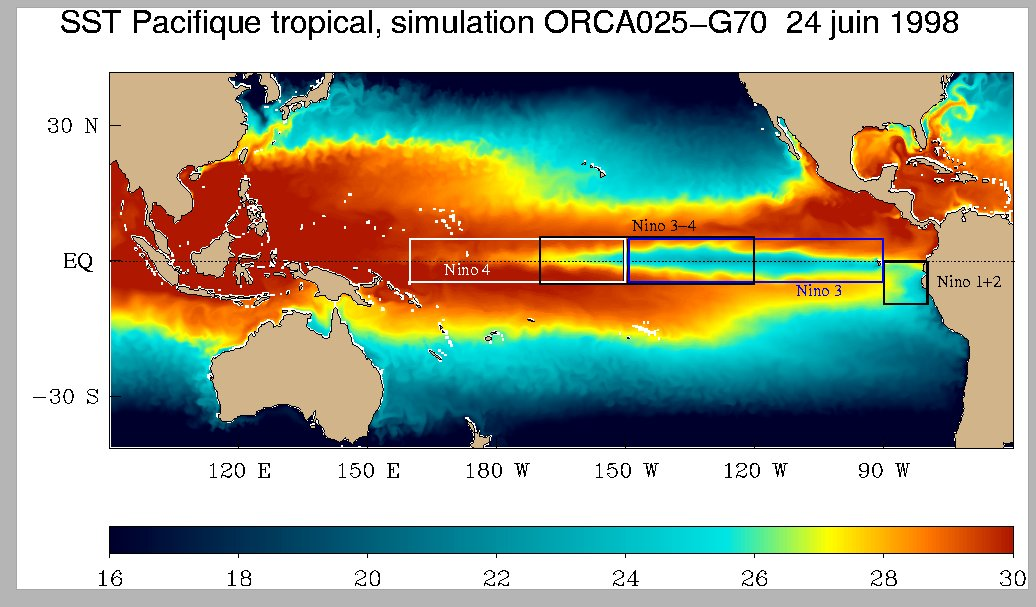
\includegraphics[width=10cm]{./figs_monitor/ninoboxes.eps}
\caption{Definition of the Nino boxes.}
\end{center}
\end{figure}

\begin{figure}[H]
\begin{center}
%\includegraphics[width=15cm]{./figs_monitor/<CONFIG>-<CASE>_nino.eps}
\caption{Monthly mean variations of the averaged temperature in el Nino boxes. Model is in black and observations (TOA array) are in green. Bottom plot is the Southern Oscillation index (monthly fluctuations in the air pressure difference between Tahiti and Darwin: sustained negative values of the SOI often indicate El Nino episodes).}
\end{center}
\end{figure}

\section*{Acknowledgement}

This simulation has been performed on Jade supercomputer (CINES) with CPU hours allocated by GENCI (\textcolor{blue}{Grant GENCI X2011XXXXXXX}).

\bibliographystyle{plain}
\bibliography{bibliographie}


\end{document}

%---------------------------------------------------------------------------------------------------



